\section{Auswertung}
\label{sec:Auswertung}

\subsection{Vorbereitung}
Bei der Vorbereitung wird für den verwendeten Kondensator und die Spule eine Eigenfrequenz von 
$f_{\text{mess}}=\SI{33.0}{\kilo\hertz}$ bei einer Phasendifferenz von $\SI{90}{\degree}$ gemessen. 
Die Referenzwerte der Bauteile lauten $C=\SI{0.8015}{\nano\farad}$ und $L=\SI{32.351}{\milli\henry}$. 
Zudem weist die Spule eine Kapazität von $C_\text{Sp}=\SI{0.037}{\nano\farad}$ auf.
Der Kondensator mit regelbarer Kapazität wird so eingestellt, dass der zweite Schwingkreis die gleiche Eigenfrequenz besitzt.

Die Anzahl der Maxima/Minima innerhalb einer (halben?) Schwebeperiode sind in der folgenden Tabelle \ref{tab:schwing_maxima} der regelbaren Kapazität $C_K$ gegenübergestellt.

\begin{table}
    \centering
    \caption{Anzahl Maxima der Schwebung.}
    \label{tab:schwing_maxima}
    \begin{tabular}{c c}
        \toprule
        {$C_K \:/\: \si{\nano\farad}$} & Schwingungsmaxima \\
        \midrule
        4.7  & 2 \\ 
        6.8  & 3 \\ 
        8.2  & 4 \\ 
        10.0 & 4 \\ 
        12.0 & 5 \\ 
        \bottomrule
    \end{tabular}
\end{table}

Im Weiteren werden die beiden Fundamentalschwingungen in Abhängigkeit der Kapazität $C_K$ bestimmt.
Für die erste Fundamentalschwingung wird bei allen Kapazitäten ein Wert von $f_- = \SI{33.1}{\kilo\hertz}$ gemessen, da der Kondensator an keinem Energieaustausch beteiligt ist.
Mit einer Phase von $\SI{180}{\degree}$ zwischen den Schwingung der beiden Schwingkreise werden jedoch von $C_K$ abhängige Werte gemessen, welche in \ref{tab:resonanz} aufgelistet sind.
Hier handelt es sich um die zweite Fundamentalschwingung.

\begin{table}
    \centering
    \caption{Resonanzfrequenzen verschiedener Kondensatoren.}
    \label{tab:resonanz}
    \begin{tabular}{c c c c c}
        \toprule
        $f_- \:/\: \si{\kilo\hertz}$ & $f_+ \:/\: \si{\kilo\hertz}$ & $C_K \:/\: \si{\nano\farad}$ & Amplitudenspannung $\:/\: \si{\milli\volt}$ & Strom $I_2 \:/\: \si{\milli\ampere}$ \\
        \midrule
        33.1 & 81.3 & 1.0  & 1830  &  38.12  \\
        33.1 & 61.1 & 2.2  & 1960  &  40.83  \\
        33.1 & 57.1 & 2.7  & 1883  &  39.22  \\
        33.1 & 48.7 & 4.7  & 2050  &  42.70  \\
        33.1 & 44.7 & 6.8  & 2160  &  45.00  \\
        33.1 & 42.8 & 8.2  & 1830  &  38.12  \\
        33.1 & 41.4 & 10.0 & 2030  &  42.29  \\
        33.1 & 40.2 & 12.0 & 2000  &  41.66  \\
        \bottomrule
    \end{tabular}
\end{table}

\begin{figure}
    \centering
    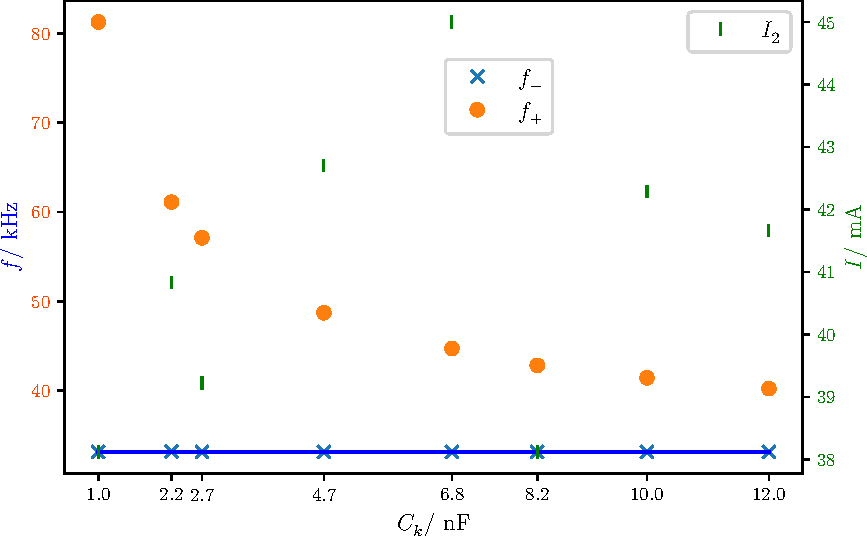
\includegraphics[width=0.75\textwidth]{plots/Messdaten.pdf}
    \caption{Die aufgenommenen Messwerte.}
    \label{fig:messwerte}
\end{figure}

Der Strom $I_2$ wird über einen Widerstand von $\SI{48}{\ohm}$ berechnet.
Zu erkennen ist die fallende Frequenz mit ansteigender Kapazität. Dies liegt an der rückstellenden Kraft der Kopplung über den Kondensator $C_K$, was in \eqref{eqn:sub} zu erkennen ist.

Die Frequenz für die erste Fundamentalschwingung errechnet sich aus 
\begin{equation}
    \label{eqn:1st_fund}
    f_+ = \frac{1}{2\pi\sqrt{LC}}
\end{equation}
und für die zweite aus
\begin{equation}
    \label{eqn:2nd_fund}
    f_- = \frac{1}{2\pi\sqrt{\frac{CC_K}{2C+C_K}}}.
\end{equation}
Um die Theoriewerte genau bestimmen zu können, werden die geringen Kapazitäten der beiden Spulen mitbeachtet.
So ergeben sich für die Gesamtkapazität je 
\begin{equation}
    C_{+, ges} = C + C_{Sp}
\end{equation}
und
\begin{equation}
    C_{-, ges} = \frac{CC_K}{2C+C_K} + C_{Sp}.
\end{equation}

Eingesetzt in \eqref{eqn:1st_fund} und \eqref{eqn:2nd_fund} berechnen sich die Werte mit
\begin{equation}
    \label{eqn:1st_fund_Csp}
    f_+ = \frac{1}{2\pi\sqrt{L(C + C_{Sp})}}
\end{equation}
\begin{equation}
    \label{eqn:2nd_fund_Csp}
    f_- = \frac{1}{2\pi\sqrt{L(\dfrac{CC_K}{2C+C_K} + C_{Sp})}}.
\end{equation}

\begin{table}
    \centering
    \caption{Die erwarteten Theoriewerte.}
    \label{tab:theorie}
    \begin{tabular}{c c c c c c c}
        \toprule
        $f_- \:/\: \si{\kilo\hertz}$ & $f_{-, theo} \:/\: \si{\kilo\hertz}$ & $f_+ \:/\: \si{\kilo\hertz}$ & $f_{+, theo} \:/\: \si{\kilo\hertz}$ & $C_K \:/\: \si{\nano\farad}$ & $I_2 \:/\: \si{\milli\ampere}$ & $I_{2,theo} \:/\: \si{\milli\ampere}$ \\
        \midrule
        33.1 & 30.5 & 81.3 & 47.6 & 1.0  &  38.12 & 19.06 \\  
        33.1 & 30.5 & 61.1 & 39.5 & 2.2  &  40.83 & 20.41 \\
        33.1 & 30.5 & 57.1 & 38.0 & 2.7  &  39.22 & 19.61 \\
        33.1 & 30.5 & 48.7 & 35.1 & 4.7  &  42.70 & 21.35 \\
        33.1 & 30.5 & 44.7 & 33.7 & 6.8  &  45.00 & 22.49 \\
        33.1 & 30.5 & 42.8 & 33.2 & 8.2  &  38.12 & 19.05 \\
        33.1 & 30.5 & 41.4 & 32.8 & 10.0 &  42.29 & 21.12 \\
        33.1 & 30.5 & 40.2 & 32.4 & 12.0 &  41.66 & 20.81 \\
        \bottomrule
    \end{tabular}
\end{table}